% Problem 1 - Residential Power Distribution Mesh Analysis (24 points)
\Point{residentialpower}{meshanalysis}{12}
\Point{residentialpower}{openneutral}{10}
\Point{residentialpower}{deviceimpact}{2}
\begin{mainquestion}{residentialpower}{Mesh Analysis}
The DC equivalent circuit of a simple residential power distribution is shown below. $R_{w}$ represents the hot wire (typically black) resistance, and $R_{n}$ represents the neutral wire (typically white) resistance. The other resistances represent loads that are drawing power: $R_{1}$ and $R_{2}$ are loads on 120 V supplies while $R_{3}$ is a load on a 240 V appliance such as a stove or a dryer.

\begin{center}
    \includegraphics[width=4in]{circuit.png}
\end{center}

\begin{partquestion}{meshanalysis}{If $R_{w}=R_{n}=0.2~\Omega$, $R_{1}=5~\Omega$, $R_{2}=12~\Omega$, and $R_{3}=13~\Omega$, use mesh analysis to determine the voltage across each of the three loads.}
\begin{answer}
Create three mesh loops in the clockwise direction for the three currents $i_{1}$ in the top-left loop, $i_{2}$ in the bottom-left loop, and $i_{3}$ in the right-hand loop. Using KVL around each loop gives:

\begin{gather*}
R_w i_1 + R_1 (i_1 - i_3) + R_n (i_1 - i_2) = 120 \\
R_w i_2 + R_2 (i_2 - i_3) + R_n (i_2 - i_1) = 120 \\
R_3 i_3 + R_1 (i_3 - i_1) + R_2 (i_3 - i_2) = 0
\end{gather*}

Then we gather like terms:

\begin{gather*}
(R_w + R_1 + R_n)i_1 - R_n i_2 - R_1 i_3 = 120 \\
- R_n i_1 + (R_w + R_2 + R_n)i_2 - R_2 i_3 = 120 \\
- R_1 i_1 - R_2 i_2 + (R_1 + R_2 + R_3)i_3 = 0
\end{gather*}

And this can be neatly written as a matrix:

\[
\begin{bmatrix}
R_w + R_1 + R_n & -R_n & -R_1 \\
-R_n & R_w + R_2 + R_n & -R_2 \\
-R_1 & -R_2 & R_3 + R_1 + R_2
\end{bmatrix}
\begin{bmatrix}
i_1 \\
i_2 \\
i_3
\end{bmatrix}
=
\begin{bmatrix}
120 \\
120 \\
0
\end{bmatrix}
\]

Substituting the given values produces:

\[
\begin{bmatrix}
5.4 & -0.2 & -5 \\
-0.2 & 12.4 & -12 \\
-5 & -12 & 30
\end{bmatrix}
\begin{bmatrix}
i_1 \\
i_2 \\
i_3
\end{bmatrix}
=
\begin{bmatrix}
120 \\
120 \\
0
\end{bmatrix}
\]

Solving these equations either by hand or some matrix solver like MATLAB gives the following:
\begin{align*}
    i_1 &= \frac{315}{8} \approx \qty{39.4}{\ampere}\\
    i_2 &= \frac{435}{16} \approx \qty{27.2}{\ampere}\\
    i_3 &= \frac{279}{16} \approx \qty{17.4}{\ampere}
\end{align*}

The voltages across the three loads are then:
\begin{align*}
v_{1} &= (i_{1}-i_{3}) R_{1} = \left( \frac{315}{8} - \frac{279}{16} \right) 5 = \frac{1755}{16} = 109.6875~\text{V} \\
v_{2} &= (i_{2}-i_{3}) R_{2} = \left( \frac{435}{16} - \frac{279}{16} \right) 12 = 117~\text{V} \\
v_{3} &= i_{3} R_{3} = \frac{279}{16} \cdot 13 = \frac{3627}{16} = 226.6875~\text{V}
\end{align*}
\end{answer}
\end{partquestion}

\begin{partquestion}{openneutral}{If a wiring fault occurs such that the neutral becomes an open circuit, recalculate the voltages across the loads.}
\begin{answer}
With the neutral open, $R_{n}\to\infty$ and the left-hand and right-hand loops remain. Let $i_{1}$ be the clockwise current in the left loop and $i_{2}$ be the clockwise current in the right loop.

The KVL system becomes:
\begin{gather*}
R_wi_1 + (R_1 + R_2)(i_1 - i_2) + R_wi_1 = 240 \\
(R_1 + R_2)(i_2 - i_1) + R_3i_2 = 0
\end{gather*}

Gather like terms:
\begin{gather*}
(2R_w + R_1 + R_2)i_1 - (R_1 + R_2)i_2 = 240 \\
- (R_1 + R_2)i_1 + (R_1 + R_2 + R_3)i_2 = 0
\end{gather*}

As a matrix:
\[
\begin{bmatrix}
2R_w + R_1 + R_2 & -R_1 -R_2\\
-R_1 -R_2 & R_1 + R_2 + R_3
\end{bmatrix}
\begin{bmatrix}
i_1 \\
i_2
\end{bmatrix}
=
\begin{bmatrix}
240 \\
0
\end{bmatrix}
\]

Substituting values yields:
\[
\begin{bmatrix}
17.4 & -17\\
-17 & 30
\end{bmatrix}
\begin{bmatrix}
i_1 \\
i_2
\end{bmatrix}
=
\begin{bmatrix}
240 \\
0
\end{bmatrix}
\]

Solving gives $i_{2} = \frac{4080}{233} \approx 17.51~\text{A}$ and $i_{1} = \frac{7200}{233} \approx 30.90~\text{A}$. The load voltages are:
\begin{align*}
v_{1} &= (i_{1}-i_{2})R_1 = \frac{15600}{233} \approx 66.95~\text{V} \\
v_{2} &= (i_{1}-i_{2})R_2 = \frac{13337}{83} \approx 160.69~\text{V} \\
v_{3} &= i_{2} R_3 = \frac{19577}{86} \approx 227.64~\text{V}
\end{align*}
\end{answer}
\end{partquestion}

\begin{partquestion}{deviceimpact}{Postulate what might happen to a sensitive device represented by $R_{2}$ if it is plugged into this faulty circuit.}
\begin{answer}
Because $R_{2}$ now sees over 160 V instead of the expected 120 V, a sensitive device is likely to be exposed to an overvoltage condition. This can damage components, cause device failure, or lead to unsafe operation.
\end{answer}
\end{partquestion}

\end{mainquestion}


% Problem 2 - Superposition with Dependent Source (10 points)
\clearpage
\Point{superposition}{calculatevx}{10}
\begin{mainquestion}{superposition}{Superposition}
Calculate $V_X$ in the circuit below using superposition.

\begin{center}
    \includegraphics[width=5.2in]{schematic.png}
\end{center}

\begin{partquestion}{calculatevx}{Use superposition to determine $V_X$.}
\begin{answer}
Superposition tells us that we can consider the effect of each independent source individually. We can do this by disabling all but one of the independent sources (open current sources, short voltage sources) and solving for $V_X$. Keep in mind you shouldn't deactivate any dependent sources. Then we can add up all the results and we should get the final value of $V_X$.

\textbf{1 A source only:} open the 2 A source and short the 3 V source. The circuit becomes:
\begin{center}
    \includegraphics[width=3in]{super_1A.png}
\end{center}

KCL at the top node gives $1 = I_X + \frac{V_X}{10}$. KVL around the outer loop gives $V_X + 4 I_X - I_X = 0$, so $I_X = -\frac{V_X}{3}$. Substituting yields:
\[
1 = -\frac{V_X}{3} + \frac{V_X}{10} = -\frac{7}{30} V_X
\]
Thus $V_X = -\frac{30}{7}~\text{V}$.

\textbf{2 A source only:} open the 1 A source and short the 3 V source. The circuit becomes:
\begin{center}
    \includegraphics[width=3in]{super_2A.png}
\end{center}

KCL gives $2 = I_X + \frac{V_X}{10}$ and the same KVL relation $I_X = -\frac{V_X}{3}$. Therefore:
\[
2 = -\frac{V_X}{3} + \frac{V_X}{10} = -\frac{7}{30} V_X
\]
so $V_X = -\frac{60}{7}~\text{V}$.

\textbf{3 V source only:} open both current sources. The circuit becomes:
\begin{center}
    \includegraphics[width=3in]{super_3V.png}
\end{center}
The remaining loop gives $I_X(1) - 4 I_X - V_X - 3 = 0$ and, because the 10~$\Omega$ resistor carries $-I_X$, $V_X = -10 I_X$. Eliminating $I_X$ yields:
\[
\frac{3 V_X}{10} - V_X - 3 = 0
\]
so $V_X = -\frac{30}{7}~\text{V}$.

Superposition sums the contributions:
\[
V_X = -\frac{30}{7} - \frac{60}{7} - \frac{30}{7} = -\frac{120}{7} \approx -17~\text{V  } (\text{well maybe $-17.14$~V})
\]
\end{answer}
\end{partquestion}

\end{mainquestion}


% Problem 3 - Ammeter Connection and Equivalent Circuits (16 points)
\clearpage
\Point{ammeter}{connection}{3}
\Point{ammeter}{thevenin}{5}
\Point{ammeter}{norton}{3}
\Point{ammeter}{ri300}{3}
\Point{ammeter}{ri0}{2}
\begin{mainquestion}{ammeter}{Equivalent Circuits}
Consider the circuit shown below. An ammeter with an internal resistance of $R_{i}$ is used to measure the current flowing through a 2 k$\Omega$ resistor between points $A$ and $B$.

\begin{center}
    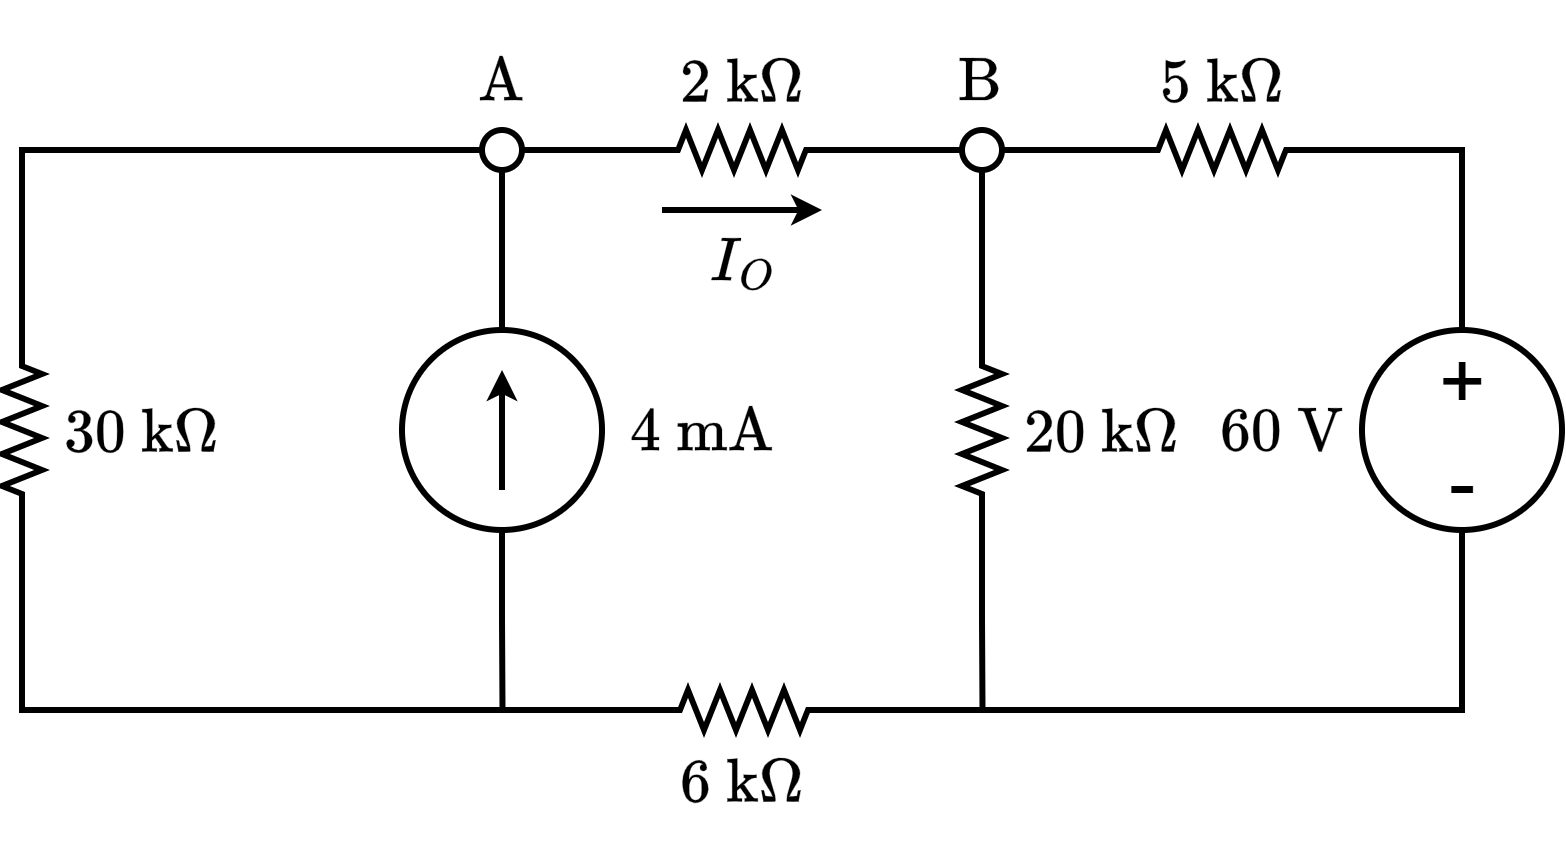
\includegraphics[width=5in]{questionbank/networks/ammeter_thevenin_norton/v0/circuit.png}
\end{center}

\begin{partquestion}{connection}{How should the ammeter be connected between $A$ and $B$? Show a sketch of the circuit (only include the portion between $A$ and $B$) which includes the ammeter with its internal resistance.}
\begin{answer}
The ammeter should be connected in series with the 2 k$\Omega$ resistor between terminals $A$ and $B$. This means the current through the load passes through the ammeter and its internal resistance.

\begin{center}
    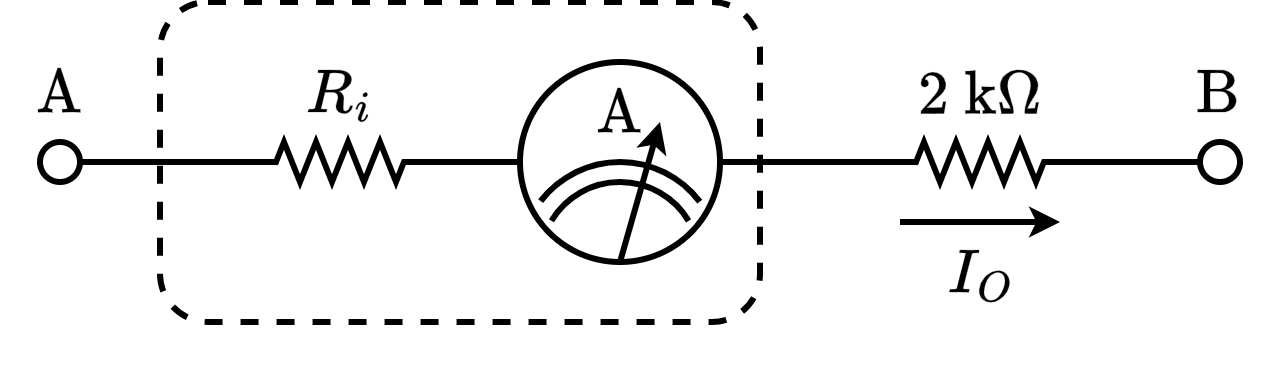
\includegraphics[width=0.7\textwidth]{questionbank/networks/ammeter_thevenin_norton/v0/ammeter_conn.png}
\end{center}
\end{answer}
\end{partquestion}

\begin{partquestion}{thevenin}{Find the Thévenin equivalent circuit at terminals $A$ and $B$ (without the 2 k$\Omega$ load).}
\begin{answer}
To find the Thévenin resistance, we zero out all independent sources. The current source becomes an open circuit and the voltage source becomes a short circuit:

\begin{center}
    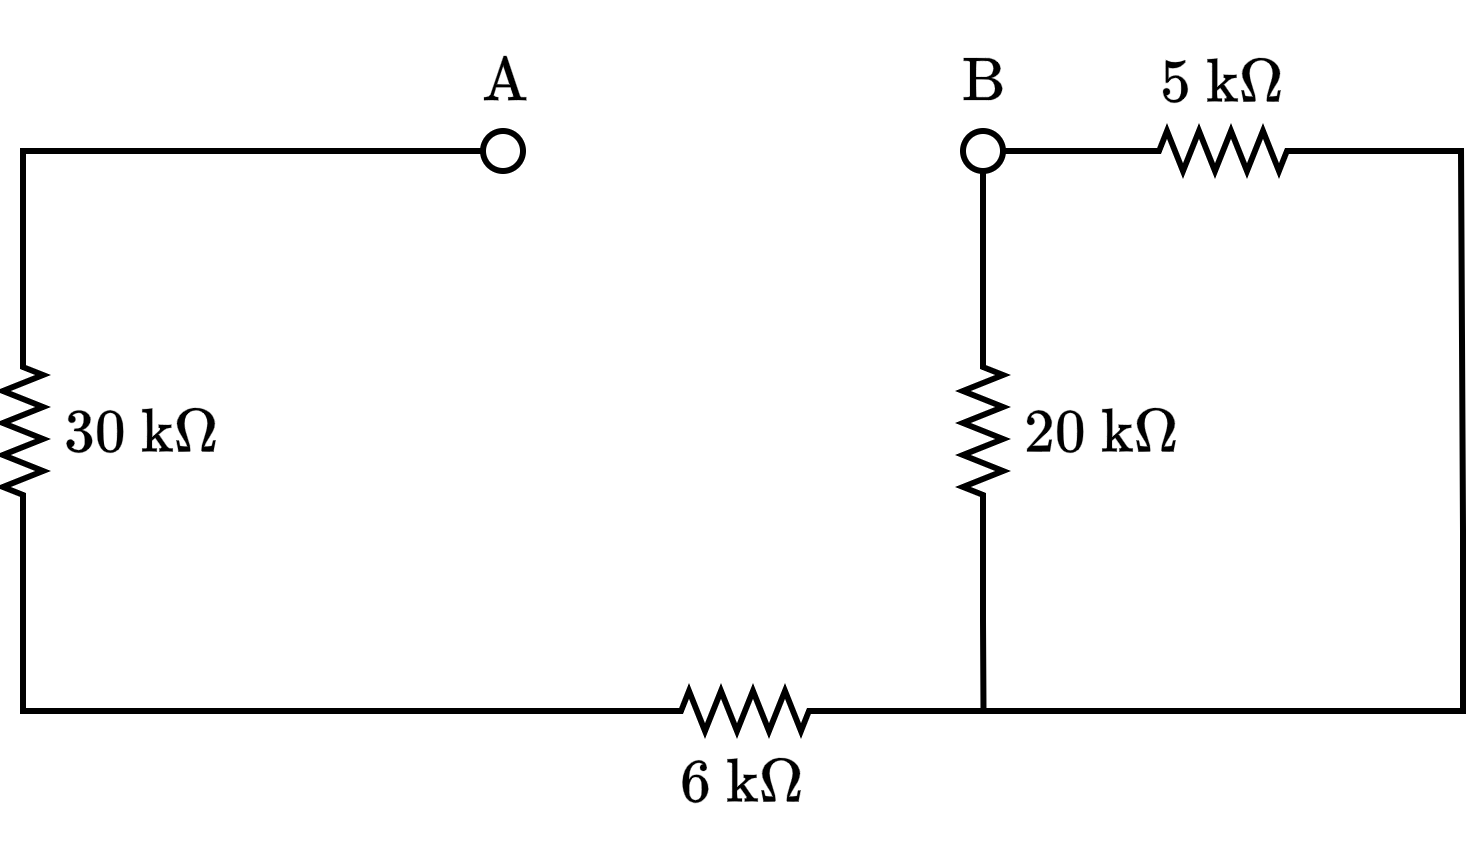
\includegraphics[width=0.7\textwidth]{questionbank/networks/ammeter_thevenin_norton/v0/rthev.png}
\end{center}

We can now combine the remaining resistors to find a single equivalent resistance.

\begin{align*}
    R_{TH} &= \qty{30}{\kilo\ohm} + \qty{6}{\kilo\ohm} + \qty{20}{\kilo\ohm}||\qty{5}{\kilo\ohm} \\
    &= \qty{36}{\kilo\ohm} + \frac{20\cdot5}{20+5}\unit{\kilo\ohm} \\
    &= \qty{40}{\kilo\ohm} \\
\end{align*}

\begin{center}
    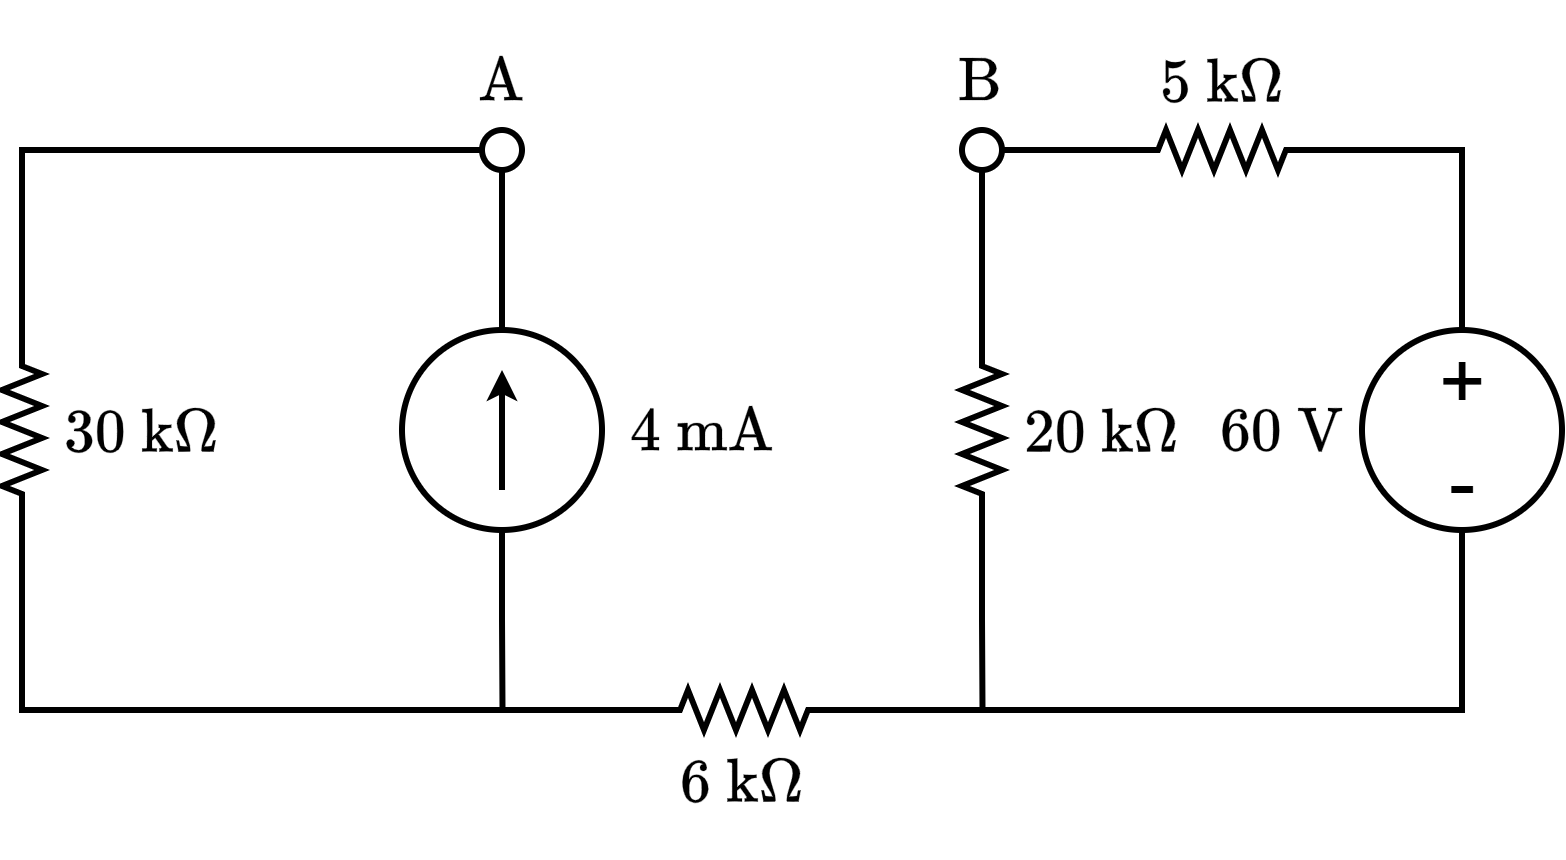
\includegraphics[width=4.5in]{questionbank/networks/ammeter_thevenin_norton/v0/thev_start.png}
\end{center}

Now to find the Thévenin voltage, compute the open-circuit voltage at $A$ and $B$. Because no current flows through the 6 k$\Omega$ branch, its voltage is zero. The open-circuit voltage measured from $A$ to $B$ is therefore the voltage drop across the current source ($\qty{4}{\milli\ampere} \cdot\qty{30}{\kilo\ohm} = \qty{120}{\volt}$) minus the output of the voltage divider formed from the \qty{20}{\kilo\ohm} and \qty{5}{\kilo\ohm} resistors with the 60 V source ($60 \frac{20}{20 +5} = \qty{48}{\volt}$). Thus $V_{\text{TH}} = 120 - 48 = 72~\text{V}$.

Now that we have both the Thévenin voltage and Thévenin resistance, we can combine them to find our equivalent circuit:

\begin{center}
    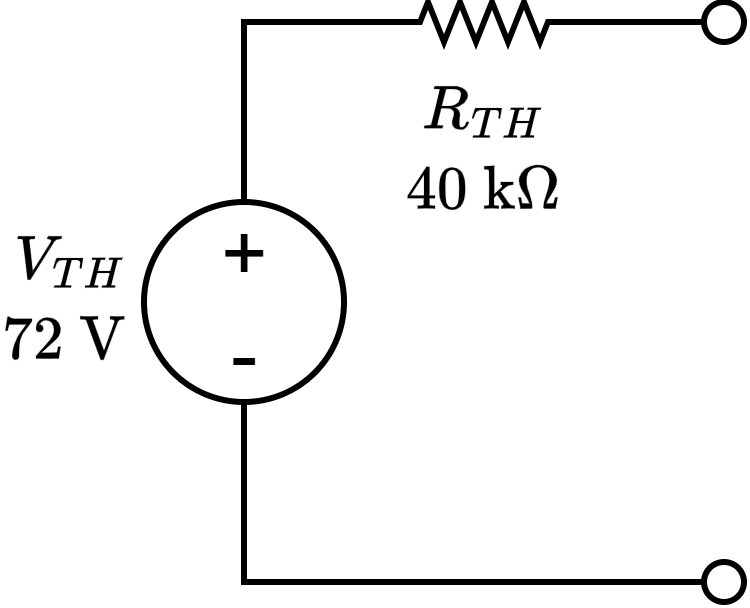
\includegraphics[width=2in]{questionbank/networks/ammeter_thevenin_norton/v0/thev_eq.png}
\end{center}
\end{answer}
\end{partquestion}

\begin{partquestion}{norton}{Find the Norton equivalent circuit at terminals $A$ and $B$ (without the 2 k$\Omega$ load).}
\begin{answer}
Using the previously computed Thévenin equivalent, the Norton current is $I_{N} = V_{\text{TH}} / R_{\text{TH}} = 72~\text{V} / 40~\text{k}\Omega = 1.8~\text{mA}$, and $R_{N} = 40~\text{k}\Omega$.

\begin{center}
    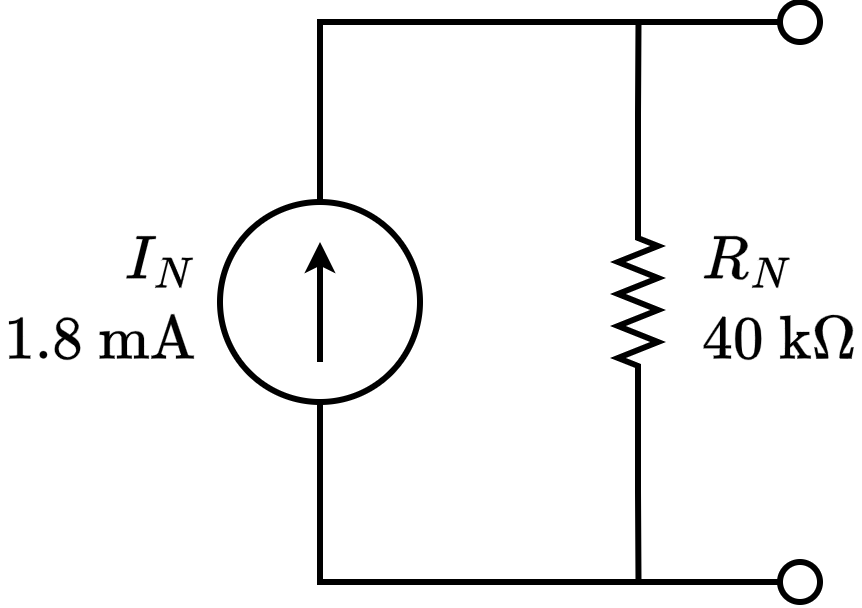
\includegraphics[width=2.2in]{questionbank/networks/ammeter_thevenin_norton/v0/norton_eq.png}
\end{center}
\end{answer}
\end{partquestion}

\begin{partquestion}{ri300}{What is the ammeter reading if $R_{i}=300~\Omega$?}
\begin{answer}
Using the Thévenin equivalent with $R_{i}=300~\Omega$ and $R_{L}=2~\text{k}\Omega$ gives:
\[
I = \frac{V_{\text{th}}}{R_{\text{th}} + R_{i} + R_{L}} = \frac{72}{40{,}000 + 300 + 2000} \approx 1.7~\text{mA}.
\]
\end{answer}
\end{partquestion}

\begin{partquestion}{ri0}{What is the reading if $R_{i}=0~\Omega$?}
\begin{answer}
With $R_{i}=0~\Omega$ the current is:
\[
I = \frac{72}{40{,}000 + 0 + 2000} \approx 1.71~\text{mA}.
\]
Note that this is not a significant deviation, and in general will not be as long as the internal resistances are kept much lower than the loads through which we wish to measure current flow.
\end{answer}
\end{partquestion}

\end{mainquestion}


% Problem 4 - Source Transformation Voltage Calculation (18 points)
\clearpage
\Point{sourcetransform}{findvo}{18}
\begin{mainquestion}{sourcetransform}{Source Transformations}
Use source transformations to find the voltage $V_{O}$ in the circuit below.

\begin{center}
    \includegraphics[width=5.2in]{circuit.png}
\end{center}

\begin{partquestion}{findvo}{Find $V_{O}$ using source transformations.}
\begin{answer}
We first transform the 3 V source with the $2~\Omega$ series resistance into its Norton equivalent with a Norton source current of $\frac{\qty{3}{\volt}}{\qty{2}{\ohm}} = \qty{1.5}{\ampere}$ and a Norton resistance of $2~\Omega$. Simultaneously, we can transform the 4 V source with the $5~\Omega$ series resistance into its Norton equivalent with a Norton source current of $\frac{\qty{4}{\volt}}{\qty{5}{\ohm}} = \qty{0.8}{\ampere}$
and a Norton resistance of $5~\Omega$. Note the polarity of the two sources are different, so the Norton current sources will be pointing in different directions! The resulting circuit looks like:

\begin{center}
    \includegraphics[width=0.8\textwidth]{transform_1.png}
\end{center}

We can simplify the circuit considerably by combining the current sources since they are in parallel to form a $\frac{17}{10}\unit{\ampere}$
source. We can also combine the three parallel resistors with a single resistor of value $\frac{15}{13}\unit{\ohm}$
The simplified circuit looks like:

\begin{center}
    \includegraphics[width=0.5\textwidth]{transform_2.png}
\end{center}

The next step is to apply another source transformation to a Thévenin equivalent with a Thévenin voltage source of $\frac{51}{26}\unit{\volt}$
with a Thévenin resistance of $\frac{15}{13}\unit{\ohm}$.
The result looks like:

\begin{center}
    \includegraphics[width=0.5\textwidth]{transform_3.png}
\end{center}

The result is a simple voltage divider. We can easily find the voltage across the $8~\Omega$ resistor as:
\[
V_{O}
=
\frac{51}{26}
\left(
\frac{8}{8+\frac{15}{13}+7}
\right)
=
\frac{34}{35}\,\si{\volt}.
\]
\end{answer}
\end{partquestion}

\end{mainquestion}

% Problem 5 - Battery Internal Resistance and Power Curve (10 points)
\clearpage
\Point{battery}{peakcurrent}{2}
\Point{battery}{peakpower}{4}
\Point{battery}{plotpower}{4}
\begin{mainquestion}{battery}{Power Transfer}
A typical CR2032 3 V coin-style battery (often used in watches or small electronic devices) has an internal source resistance $R_{s}$ of about $17~\si{\ohm}$ (seriously!) at room temperature. (While this value typically increases as the battery is depleted, we will consider it constant for this problem.)

\begin{center}
    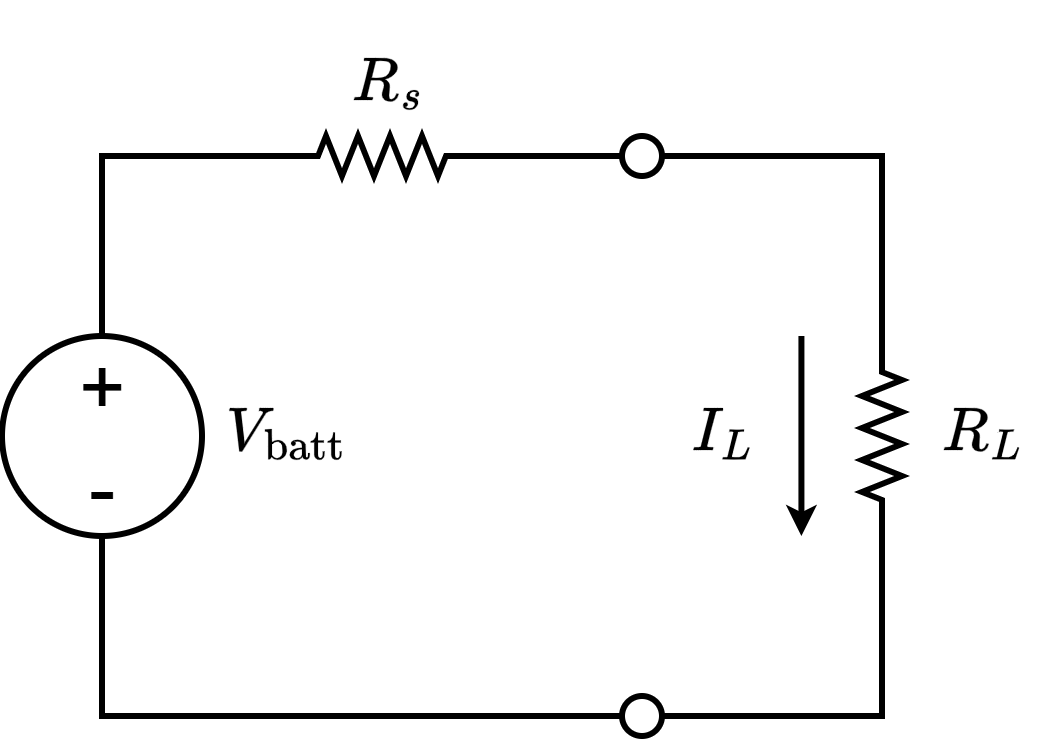
\includegraphics[width=4in]{questionbank/networks/battery_internal_resistance/v0/circuit.png
    }
\end{center}

\begin{partquestion}{peakcurrent}{Using this battery, what is the peak current that could be driven through an external load $R_{L}$? What is $R_{L}$ in this scenario?}
\begin{answer}
The current is
\[
I=\frac{V_{\text{batt}}}{R_s+R_L},
\]
and to make this as large as possible, we make the denominator as small as possible. With $R_s$ fixed, we make
\[
R_L=0,
\]
so
\[
I=\frac{V_{\text{batt}}}{R_s} = \frac{3}{17}\,\si{\ampere}
    \approx 176\,\si{\milli\ampere}.
\]
\end{answer}
\end{partquestion}

\begin{partquestion}{peakpower}{Using this battery, what is the peak power that could be delivered through an external load $R_{L}$? What is $R_{L}$ in this scenario?}
\begin{answer}
Maximum power transfer occurs when
\[
R_L=R_s=17\,\si{\ohm},
\]
and the value of the power is
\[
P= \frac{V_L^2}{R_L} = \frac{(V_{\text{batt}}\frac{R_L}{R_s + R_L})^2}{R_L} = \frac{V_{\text{batt}}^2R_L}{(R_s + R_L)^2}
= \frac{V_{\text{batt}}^2}{4R_s}
=\frac{3^2}{4(17)}
=\frac{9}{68}\,\si{\watt}
\approx132\,\si{\milli\watt}.
\]
\end{answer}
\end{partquestion}

\begin{partquestion}{plotpower}{Plot the power delivered to $R_{L}$ as a function of $R_{L}$, from $0$ to $500~\si{\ohm}$.}
\begin{answer}
In the previous part, we derived the formula for the power dissipated in the load as:
\[P_{L} = \frac{V_{\text{batt}}^{2} R_{L}}{(R_{L} + R_{s})^{2}} = \frac{9 R_{L}}{(R_{L} + 17)^{2}}.\]

This can be plotted using MATLAB or some equivalent graphing program; the figure is shown below.

\begin{center}
    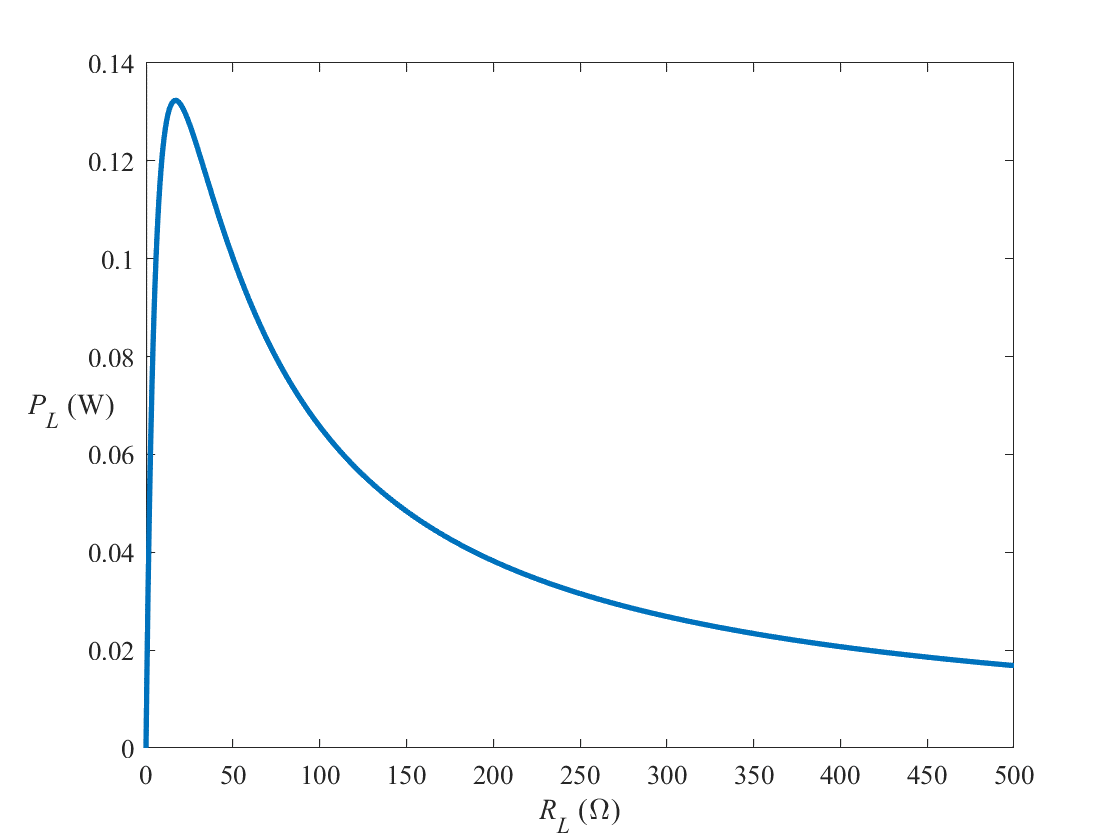
\includegraphics[width=5in]{questionbank/networks/battery_internal_resistance/v0/plot.png}
\end{center}

Note the peak occurs at $17~\si{\ohm}$, as we expect. The power delivered to the load rolls off to zero as $R_L$ goes to zero.
\end{answer}
\end{partquestion}

\end{mainquestion}
